% This work is licensed under the Creative Commons Attribution-NonCommercial-NoDerivs
% 3.0 Unported License. To view a copy of this license, visit
% http://creativecommons.org/licenses/by-nc-nd/3.0/ or send a letter to
% Creative Commons, 444 Castro Street, Suite 900, Mountain View, California, 94041, USA.

%-------------------------------------------------------------------------------
\begin{frame}[fragile]\frametitle{Mises à jour du dépôt local}
  \begin{itemize}
    \item S'informer des changements distants: \alert{git fetch}
    \item Fetch et appliquer dans le repository local : \alert{git pull}
  \end{itemize}

\end{frame}
%-------------------------------------------------------------------------------
\begin{frame}[fragile]\frametitle{Mises à jour du dépôt local, fast forward}
  \begin{center}
    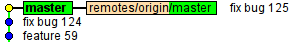
\includegraphics[width=0.8\textwidth]{./images/merge-0.png}
  \end{center}
  \pause
  \hfill
  \begin{center}
    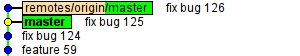
\includegraphics[width=0.8\textwidth]{./images/merge-1.png}
  \end{center}
  \pause
  \hfill
  \begin{center}
    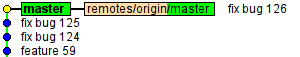
\includegraphics[width=0.8\textwidth]{./images/merge-2.png}
  \end{center}
\end{frame}
%-------------------------------------------------------------------------------
\begin{frame}[fragile]\frametitle{Mises à jour du dépôt local, non fast forward}
  \begin{center}
    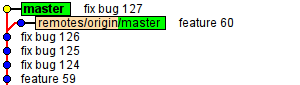
\includegraphics[width=0.8\textwidth]{./images/merge-3.png}
  \end{center}
  \pause
  \hfill
  \begin{center}
    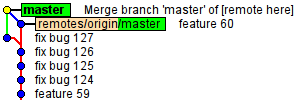
\includegraphics[width=0.8\textwidth]{./images/merge-4.png}
  \end{center}
\end{frame}
%-------------------------------------------------------------------------------
\begin{frame}[fragile]\frametitle{Mises à jour du dépôt distant}
  \alert{git push}
  \hfill
  \begin{center}
    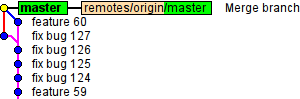
\includegraphics[width=0.8\textwidth]{./images/merge-5.png}
  \end{center}
  \note{attention au push.default, qui a changé avec git 1.7.11}
\end{frame}
%-------------------------------------------------------------------------------
\begin{frame}\frametitle{TP}
  git pull, commit, push
\end{frame}
%-------------------------------------------------------------------------------
% max 80 columns : merges become messy with pure text and longer lines.
% vim: set colorcolumn=+1 textwidth=80:
